% T12 C/D, chapitre 5 : Barycentres. Source : le livre « Terminales scientifiques » (Barycentre/Lesona, Barycentre/Exo).
% Les exercices tirés d’autres ouvrages ne sont pas repris (décision du 2 novembre 2026).

\TCDLessonStyleOn
\providecommand{\D}{\mathcal{D}}

\begin{chapter}{Calcul barycentrique}
\index{Barycentre}
\section{Barycentre de $n$ points pond\'er\'es}

\begin{defi}[Point pond\'er\'e]
On appelle \emph{point pond\'er\'e} tout couple de la forme $(A,\alpha)$ o\`u $A$ est un point et $\alpha$ un nombre r\'eel.
Le nombre r\'eel $\alpha$ est appell\'e \emph{coefficient} de $A$.
\end{defi}

\subsection{Barycentre de deux points pond\'er\'es}
\index{Barycentre!de deux points}
Soient $(A,\alpha)$ et $(B,\beta)$ deux points pond\'er\'es tels que $A \neq B$ et $\alpha + \beta \neq 0$.
On appelle \emph{barycentre} du syst\`eme $\{ (A,\alpha) ; (B,\beta) \}$ le point $G$ qui v\'erifie 
\defbox{$\alpha \; \overrightarrow{GA} + \beta \; \overrightarrow{GB} = \vec{0}$}.

\subsection{Coordonn\'ees du barycentre}
Dans le plan $(O, \vec{\imath} , \vec{\jmath})$, soit $\{ (A,\alpha) ; (B,\beta) \}$ un syst\'eme pond\'er\'e non nul et soit $G$ le barycentre de ce syst\'eme.

On sait que $ \alpha \overrightarrow{GA} + \beta \overrightarrow{GB} = \vec{0}$.
A l'aide de la relation de Chasles, on a
\begin{align*}
\alpha ( \overrightarrow{GO} + \overrightarrow{OA} ) + \beta ( \overrightarrow{GO} + \overrightarrow{OB} ) & = \vec{0} \\
(\alpha + \beta) \overrightarrow{GO} + \alpha \overrightarrow{OA} + \beta \overrightarrow{OB} & = \vec{0} \\
\intertext{ainsi}
\overrightarrow{OG} = \frac{\alpha \overrightarrow{OA} + \beta \overrightarrow{OB}}{\alpha + \beta} \label{eq:barycentre coordonnees vecteurs}
\end{align*}

Posons $(x_a , y_a)$, $(x_b , y_b)$ et $(x_g , y_g)$ les coordonn\'ees respectives de $A$, $B$ et $G$.
\begin{equation}
\label{eq:barycentre coordonnees composantes}
\veccor{x_g}{y_g} = \frac{1}{\alpha + \beta} \left[ \alpha  \veccor{x_a}{y_a}  + \beta \veccor{x_b}{y_b} \right]
\end{equation}

Ainsi, 
$$
\left\lbrace
\begin{matrix}
x_g = \frac{1}{\alpha + \beta} \; (\alpha x_a + \beta x_b) \\ 
\\
y_g = \frac{1}{\alpha + \beta} \; (\alpha y_a + \beta y_b) 
\end{matrix}
\right.
$$

\begin{exe} ~ \newline \vspace{-.2cm} \newline
\label{exe:barycentre 1}
%
On rapporte le plan \`a un rep\`ere orthonorm\'e $(O , \vec{\imath} , \vec{\jmath})$. 
Soient $A (1,-1)$ et $B(2,1)$ deux points du plan.
Placez $A$, $B$ et $G = \mathrm{bar}\left\lbrace (A,1) ; (B,-2) \right\rbrace $ 
dans le plan.

Avant de placer ces points dans un rep\`ere orthonorm\'e, il nous faut d'abord calculer les coordonn\'ees du point $G$.
D'apr\`es l'\'equation~\eqref{eq:barycentre coordonnees composantes}, on a \newline
\begin{minipage}{0.55\actualtextwidth}
%\begin{equation}
%x_g = \frac{1}{(1 + (-2))} (1 \cdot 1 + (-2) \cdot 2)    
%    = \frac{1}{-1} (1-4)                                 
%    = 3                                                  
%\end{equation}
%et
%\begin{equation}
%y_g = \frac{1}{(1 + (-2))} (1 \cdot (-1) + (-2) \cdot 1) 
%    = \frac{1}{-1} (-1 - 2)                              
%    = 3                                                  \; .
%\end{equation}
% Io ambony io ihany ito ambany ito fa version align fotsiny %
\begin{align*}
x_g & = \frac{1}{(1 + (-2))} (1 \cdot 1 + (-2) \cdot 2)    \\
    & = \frac{1}{-1} (1-4)                                 \\
    & = (-1) \cdot (-3)                                    \\
    & = 3                                                  \\
\intertext{et }
y_g & = \frac{1}{(1 + (-2))} (1 \cdot (-1) + (-2) \cdot 1) \\
    & = \frac{1}{-1} (-1 - 2)                              \\
    & = (-1) (-3)                                          \\
    & = 3
\end{align*}
Ainsi, $x_g = 3 $ et $y_g = 3$.
\end{minipage}
%
\begin{minipage}{.4\actualtextwidth}
	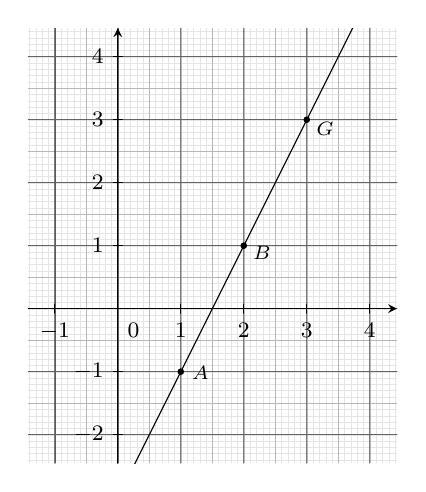
\begin{tikzpicture}[scale = .8 , line cap=round,line join=round,>=stealth,x=1.0cm,y=1.0cm]
		\draw [color=black, xstep=.1,ystep=.1, opacity=.1, line width=.1] (-1.42,-2.45) grid (4.43,4.45);
		\draw [color=black, xstep=.5,ystep=.5, opacity=.2, line width=.2] (-1.42,-2.45) grid (4.43,4.45);
		\draw [color=black, xstep=1,ystep=1, opacity=.5, line width=.5] (-1.42,-2.45) grid (4.43,4.45);
		\draw[->,color=black] (-1.42,0) -- (4.43,0);
		\foreach \x in {-1,1,2,3,4}
		\draw[shift={(\x,0)},color=black] (0pt,2pt) -- (0pt,-2pt) node[below] {\footnotesize $\x$};
		\draw[->,color=black] (0,-2.45) -- (0,4.45);
		\foreach \y in {-2,-1,1,2,3,4}
		\draw[shift={(0,\y)},color=black] (2pt,0pt) -- (-2pt,0pt) node[left] {\footnotesize $\y$};
		\draw[color=black] (0pt,-10pt) node[right] {\footnotesize $0$};
		\clip(-1.42,-2.45) rectangle (4.43,4.45);
		\draw [domain=-1.42:4.43] plot(\x,{(--3-2*\x)/-1});
		\begin{scriptsize}
			\fill [color=black] (1,-1) circle (1.5pt);
			\draw[color=black] (1.31,-1.02) node {$A$};
			\fill [color=black] (2,1) circle (1.5pt);
			\draw[color=black] (2.29,0.88) node {$B$};
			\fill [color=black] (3,3) circle (1.5pt);
			\draw[color=black] (3.29,2.85) node {$G$};
		\end{scriptsize}
	\end{tikzpicture}
\end{minipage}
\end{exe}
%
\subsection{Propri\'et\'es du barycentre pour deux points pond\'er\'es}
\begin{prop}[Colin\'earit\'e]
	Si $G$ est le barycentre du syst\`eme pond\'er\'e non nul $\{ (A,\alpha) , (B,\beta) \}$ 
	alors $G$ appartient \`a la droite $(AB)$.
	
	Si, de plus, $G$ appartient au segment $[AB]$ et est distinct de $A$ et de $B$, alors $\alpha$ et $\beta$ sont non nuls et de m\^eme signe.
%
	\begin{proof}
		Comme $G$ est le barycentre du syst\`eme pond\'er\'e $\{ (A,\alpha) , (B,\beta) \}$, 
		alors $\alpha \overrightarrow{GA} + \beta \overrightarrow{GB} = \vec{0}$.
		Si $\alpha = 0$, alors $\beta \neq 0$ et $\beta \overrightarrow{GB} = \vec{0}$, donc $G = B$, qui appartient \`a $(AB)$.
		Supposons d\'esormais $\alpha \neq 0$ ; l'\'egalit\'e pr\'ec\'edente nous donne $\alpha \overrightarrow{GA} = -\beta \overrightarrow{GB}$
		ou encore $\overrightarrow{GA} = - \frac{\beta}{\alpha} \overrightarrow{GB}$
		ce qui prouve que $\overrightarrow{GA}$ et $\overrightarrow{GB}$ sont colin\'eaires, donc que $G$ appartient \`a la droite $(AB)$.
		
		Si, de plus, $G \in [AB]$ avec $G \neq A$ et $G \neq B$, alors $\alpha \neq 0$ (sinon $G = B$), $\beta \neq 0$ (sinon $G = A$), et $\overrightarrow{GA}$ et $\overrightarrow{GB}$ 
		sont non nuls et de sens oppos\'es ce qui se traduit par le fait que 
		$\overrightarrow{GA} = k \overrightarrow{GB}$ o\`u $k$ est un nombre n\'egatif.
		Comme on sait que $\overrightarrow{GA} = - \frac{\beta}{\alpha} \overrightarrow{GB}$, 
		alors $- \frac{\beta}{\alpha}$ est un nombre n\'egatif ; cela entra\^ine que  
		$\frac{\beta}{\alpha}$ est de signe positif et donc que $\alpha$ et $\beta$ sont de m\^eme signe.
	\end{proof}
\end{prop}
%
\begin{prp}
	Soient $A$ et $B$ deux points distincts et $\D$ la droite $(AB)$.
	\begin{itemize} 
		\item Tout point de $\D$ peut s'\'ecrire comme barycentre des points $A$ et $B$.
		\item Pour un point $M$ de $\D$, il existe plusieurs mani\'eres d'\'ecrire $M$ comme barycentre de $A$ et $B$.
	\end{itemize}
	%
	\begin{proof}
		\begin{itemize} 
		\item Soit $M$ un point de la droite $\D$.
			Comme $A$, $B$ et $M$ sont colin\'eaire, 
			il existe un r\'eel $\mu$ tel que $\overrightarrow{AM} = \mu \overrightarrow{AB}$
			en utilisant la relation de Chasles,
			on a $\overrightarrow{AM} = \mu (\overrightarrow{AM} + \overrightarrow{MB})$
			et donc $ \vec{0} = \mu \overrightarrow{AM} + \mu \overrightarrow{MB} + \overrightarrow{MA} $
			puis $\vec{0} = \overrightarrow{MA} - \mu \overrightarrow{MA} + \mu \overrightarrow{MB}$
			et enfin, $(1-\mu) \overrightarrow{MA} + \mu \overrightarrow{MB} = \vec{0}$.
			Comme $(1-\mu) + \mu = 1 \neq 0$, donc on peut prendre $\alpha = (1-\mu)$ et $\beta = \mu$ ; 
			on a alors $\alpha \overrightarrow{MA} + \beta \overrightarrow{MB} = \vec{0}$ 
			ce qui signifie que $M$ est un barycentre de $A$ et $B$.
		\item Soit maintenant $G$ le barycentre du syst\`eme $\{ (A,\alpha) ; (B,\beta) \}$.
			Cela signifie que $\alpha \overrightarrow{GA} + \beta \overrightarrow{GB} = \vec{0}$.
			Si $\gamma$ est un nombre r\'eel non-nul, 
			alors $\gamma \alpha \overrightarrow{GA} + \gamma \beta \overrightarrow{GB} = \vec{0}$.
			Ainsi, $G$ est aussi le barycentre du syst\'eme $\{ (A,\gamma \alpha) ; (B,\gamma \beta) \}$.
		\end{itemize}
	\end{proof}
\end{prp}
%
Si $M$ est le barycentre du syst\`eme $\{ (A, \alpha) ; (B, \beta) \}$, alors le couple $(\alpha,\beta)$ constitue les \emph{coordonn\'ees barycentriques} de $M$ par rapport \`a $(A,B)$.
%
\subsection{Barycentre de trois points pond\'er\'es}
\index{Barycentre!de trois points}
%
\begin{defi}
Etant donn\'e un syst\`eme de trois points pond\'er\'es $\{ (A, \alpha) ; (B, \beta) ; (C, \gamma) \}$ tel que 
$\alpha + \beta + \gamma \neq 0$,
on appelle barycentre du syst\`eme le point $M$ du plan tel que $\alpha \overrightarrow{MA} + \beta \overrightarrow{MB} + \gamma \overrightarrow{MC} = \vec{0}$.
\end{defi}

Montrons que tout syst\`eme de cette forme admet un barycentre. \\
Notons par $\mathcal{P}$ le plan euclidien et par $\overrightarrow{\mathcal{P}}$ le plan vectoriel.
Soit $\vec{f}$ l'application de $\mathcal{P}$ vers $\overrightarrow{\mathcal{P}}$ qui, \`a tout point $M$ de $\mathcal{P}$,
associe le vecteur $\alpha \overrightarrow{MA} + \beta \overrightarrow{MB} + \gamma \overrightarrow{MC}$.
On veut alors conna\^itre les solutions de l'\'equation $\vec{f}(M) = \vec{0}$.

Prenons un point $N$ de $\mathcal{P}$.
D'apr\`es la relation de Chasles, on a \\
\begin{align*}
\vec{f}(M) & = \alpha \overrightarrow{MN} + \alpha \overrightarrow{NA} + \beta \overrightarrow{MN} + \beta \overrightarrow{NB} + \gamma \overrightarrow{MN} + \gamma \overrightarrow{NC} \\
           & = (\alpha + \beta + \gamma) \overrightarrow{MN} + \vec{f}(N)      \; .
\end{align*}
\begin{itemize} 
\item Si $\alpha + \beta + \gamma = 0$ alors $\vec{f}(M) = \vec{f}(N)$ pour tout $M$ et $N$ de $\mathcal{P}$ et la fonction $\vec{f}$ est donc constante%
\footnote{\'egal \`a $\beta \overrightarrow{AB} + \gamma \overrightarrow{AC}$}.
\item Si $\alpha + \beta + \gamma \neq 0$, fixons un origine qu'on appellera $O$.
      On a alors
      \begin{align*}
      \vec{f}(G) & = (\alpha + \beta + \gamma) \overrightarrow{GO} + \overrightarrow{f(O)} \\
                 & = (\alpha + \beta + \gamma) \overrightarrow{GO} + \alpha \overrightarrow{OA} + \beta \overrightarrow{OB} + \gamma \overrightarrow{OC} \\
      \intertext{et si $G$ est le barycentre alors $\vec{f}(G) = \vec{0}$ et on a }
      \vec{0} & = (\alpha + \beta + \gamma) \overrightarrow{GO} + \alpha \overrightarrow{OA} + \beta \overrightarrow{OB} + \gamma \overrightarrow{OC} \\
      \intertext{et ainsi}
      \end{align*}
\propbox{$$\overrightarrow{OG} = \frac{ \alpha \overrightarrow{OA} + \beta \overrightarrow{OB} + \gamma \overrightarrow{OC} }{ \alpha + \beta + \gamma } \; .$$}
\end{itemize}
%
\begin{thm}
Si $\alpha + \beta + \gamma \neq 0$, alors il existe un unique point $G$ tel que $\alpha \overrightarrow{GA} + \beta \overrightarrow{GB} + \gamma \overrightarrow{GC} = \vec{0}$.
Ce point $G$ est appel\'e \emph{barycentre} du syst\`eme $((A,\alpha),(B,\beta),(C,\gamma))$.
\end{thm}
%
\subsubsection{Coordonn\'ees du barycentre}
On rapporte maintenant le plan $\mathcal{P}$ \`a un rep\`ere $(O,\vec{\imath},\vec{\jmath})$.
Soit $((A,\alpha),(B,\beta),(C,\gamma))$ un syst\`eme de points pond\'er\'es tel que $\alpha + \beta + \gamma \neq 0$.
Soient $(x_A , y_A)$, $(x_B , y_B)$ et $(x_C , y_C)$ les coordonn\'ees respectives de $A$, $B$ et $C$.
Soit $G (x_G , y_G)$ le barycentre du syst\`eme.
Comme $\overrightarrow{OG} = \frac{\alpha \overrightarrow{OA} + \beta \overrightarrow{OB} + \gamma \overrightarrow{OC}}{\alpha + \beta + \gamma}$, on a 
\[
\left\lbrace
\begin{matrix}
x_G = \frac{\alpha x_A + \beta x_B + \gamma x_C }{\alpha + \beta + \gamma} \\
y_G = \frac{\alpha y_A + \beta y_B + \gamma y_C }{\alpha + \beta + \gamma} \; .
\end{matrix}
\right.
\]
Tout triplet $(\alpha , \beta , \gamma)$ tel que $M$ soit un barycentre de $((A,\alpha),(B,\beta),(C,\gamma))$ constitue des \emph{coordonn\'ees barycentriques}.
%
\subsubsection{Associativit\'e du barycentre}
\index{Barycentre!associativite@associativit\'e}
Soient les deux syst\`emes de points pond\'er\'es non nuls
\[
  \begin{aligned}
    \mathcal{S}  &= ((A,\alpha),(B,\beta),(C,\gamma)), \\
    \mathcal{S}' &= ((A,\alpha),(B,\beta)).
  \end{aligned}
\]
On note $G$ le barycentre de $\mathcal{S}$ et $G'$ celui de $\mathcal{S}'$.
\par\noindent
\propbox{Alors $G$ est aussi le barycentre du syst\`eme
$\left((G',\alpha+\beta),(C,\gamma)\right)$.}
%
\begin{proof}
En effet, avec ces hypoth\`eses on a $\alpha \overrightarrow{G' A} + \beta \overrightarrow{G' B} = \vec{0}$ ce qui, d'apr\`es la relation de Chasles, donne 
$\alpha \overrightarrow{GA} + \beta \overrightarrow{GB} = (\alpha + \beta) \overrightarrow{GG'}$.
Combinant cette derni\`ere avec l'\'egalit\'e $\alpha \overrightarrow{GA} + \beta \overrightarrow{GB} + \gamma \overrightarrow{GC} = \vec{0}$, on a 
$(\alpha + \beta) \overrightarrow{GG'} + \gamma \overrightarrow{GC} = \vec{0}$ ce qui montre que $G$ est le barycentre du syst\`eme $((G' , \alpha + \beta),(C , \gamma))$.
\end{proof}
%
\subsection{Barycentre de $n$ points pond\'er\'es}
\index{Barycentre!de n points@de $n$ points}
%
Le barycentre de $n$ points pond\'er\'es n'est autre qu'une g\'en\'eralisation du barycentre de trois points pond\'er\'es.
      \begin{defi}
            Soient $A_1,\ A_2,\ \ldots ,\ A_n$ $n$ points distincts du plan.
            Soient $\alpha_1,\ \alpha_2,\ \ldots ,\ \alpha_n$ $n$ nombres r\'eels.
            
            Si $\alpha_1 + \alpha_2 + \cdots + \alpha_n \neq 0$ alors il existe un unique point $G$ 
            tel que $\alpha_1 \overrightarrow{GA_1} + \alpha_2 \overrightarrow{GA_2} + \cdots + \alpha_n \overrightarrow{GA_n} = \vec{0}$.
            
	            Le point $G$ ainsi d\'efini est appel\'e \emph{barycentre} du syst\`eme 
	            \[
	              \left\lbrace (A_1,\alpha_1) ; (A_2,\alpha_2) ; \ldots ; (A_n,\alpha_n) \right\rbrace.
	            \]
      \end{defi}
      %
      \begin{prop}
            Soient 
            $\left\lbrace (A_1,\alpha_1) ; (A_2,\alpha_2) ; \ldots ; (A_n,\alpha_n) \right\rbrace$
            un syst\`eme de points pond\'er\'es v\'erifiant $\sum \alpha_i \neq 0$ et soit $G$ le barycentre de ce syst\`eme.
            
            \begin{enumerate}
                  \item le barycentre $G$ est ind\'ependant de l'ordre des couples $(A_i , \alpha_i)$,
	                  \item pour tout r\'eel non nul $k$, le point $G$ est aussi le barycentre du syst\`eme 
	                        \[
	                          \left\lbrace (A_1,k\alpha_1) ; (A_2,k\alpha_2) ; \ldots ; (A_n,k\alpha_n) \right\rbrace,
	                        \]
                  \item \index{Barycentre!isobarycentre}
\index{centre de gravite@centre de gravit\'e}
                        si $\alpha_1 = \alpha_2 = \cdots = \alpha_n$, on dit que $G$ est 
                        l'\emph{isobarycentre} ou le centre de gravit\'e des points 
                        $A_1,\ A_2,\ \ldots ,\ A_n$,
                  \item \label{prop: associativite}
                        si $p<n$ et que $\alpha_1 + \alpha_2 + \cdots + \alpha_p = \alpha' \neq 0$, alors 
	                        le syst\`eme 
	                        \[
	                          \left\lbrace (A_1,\alpha_1) ; (A_2,\alpha_2) ; \ldots ; (A_p,\alpha_p) \right\rbrace
	                        \]
                        admet un barycentre $G'$.
	                        Le point $G$ est aussi le barycentre du syst\`eme 
	                        \[
	                          \left\lbrace (G',\alpha') ; (A_{p+1},\alpha_{p+1}) , \ldots , (A_n,\alpha_n) \right\rbrace.
	                        \]
            \end{enumerate}
            %
            \smallnota{Comme l'ordre des couples ne change pas le barycentre,
                       le point $G'$ de \ref{prop: associativite} peut \^etre remplac\'e par
                       le barycentre de n'importe quel sous-ensemble de $p$ couples, 
                       et non seulement des $p$ premiers.
                       }
      \end{prop}
%
\section{Fonctions de Leibniz}
%
\subsection{Fonction vectorielle de Leibniz}
\index{Leibniz!Fonction vectorielle de}
%
On consid\`ere l'espace affine $E$ associ\'e \`a l'espace vectoriel $V$. 
Soit $(A_i , \alpha_i)_{i = 1 , \dots , n}$ une famille de points pond\'er\'es.
\begin{defi} ~ \newline
On appelle \emph{fonction vectorielle de Leibniz} associ\'ee au syst\`eme
$\{(A_i,\alpha_i)\}_{i=1,\dots,n}$ l'application de $E$ dans $V$ qui, \`a tout point $M$, associe le vecteur
	\defbox{
		$$
			\vec{f}(M) = \sum_{i = 1}^{n} \alpha_i \overrightarrow{MA_i}
			\; .
		$$
	}
\end{defi}
%
Posons $m = \sum_{i = 1}^{n} \alpha_i$.
%
\begin{prp}
	\label{prp:f(M) = f(N) + m MN}
	Pour tout couple de points $(M , N)$, on a 
		\propbox{
			$$   \vec{f}(M) = \vec{f}(N) + m \; \overrightarrow{MN}		\; .$$
		}
	%
	\begin{proof}
		Soit $(M,N)$ un couple de points de $E$.
		D'apr\`es la relation de Chasles, on a 
			\begin{displaymath}
			\vec{f}(M) = \sum_{i = 1}^n \alpha_i ( \overrightarrow{MN} + \overrightarrow{NA_i} ) 
				= \sum_{i = 1}^n \alpha_i  \overrightarrow{MN} + \sum_{i = 1}^n \alpha_i \overrightarrow{NA_i} 
				= \left( \sum_{i = 1}^n \alpha_i \right) \cdot \overrightarrow{MN} + \vec{f}(N)           
			\; .
			\end{displaymath}
	\end{proof}
\end{prp}
%
\begin{prp} \label{prp:fonction vectorielle}
	Selon la valeur de $\sum_{i = 1}^{n} \alpha_i$, on distingue deux cas : 
	\begin{enumerate}
	\item \textbf{Si $\boldsymbol{\sum_{i = 1}^{n} \alpha_i = 0}$ } alors la fonction $\vec{f}$ est constante.
	\item \label{prp: fonction vectorielle 2}
		\textbf{Si $\boldsymbol{\sum_{i = 1}^{n} \alpha_i \neq 0}$ } alors il existe un point $G$ tel que $\vec{f}(G) = \vec{0}$. De plus, pour tout point $M$ on a $\vec{f}(M) = (\sum_{i = 1}^{n} \alpha_i) \; \overrightarrow{MG}$.
	\end{enumerate}
	\begin{proof}
		\begin{enumerate}
			\item Supposons que $\sum_{i = 1}^{n} \alpha_i = 0$. 
				Soient $M$ et $N$ deux points.
				D'apr\`es la Propri\'et\'e~\ref{prp:f(M) = f(N) + m MN}, 
				on a $\vec{f}(M) = \vec{f}(N) + m \; \overrightarrow{MN}$.
				Comme $m = 0$ alors $\vec{f}(M) = \vec{f}(N)$.
				On d\'eduit que $\vec{f}$ est constante.
			\item Supposons que $\sum_{i = 1}^{n} \alpha_i \neq 0$. 
				Fixons un point $O$ comme origine. 
				D'apr\`es la Propri\'et\'e~\ref{prp:f(M) = f(N) + m MN}, 
				pour tout point $M$ on a $\vec{f}(M) = \overrightarrow{f(O)} + m \; \overrightarrow{MO}$.
				Cette propri\'et\'e est en particulier vraie pour le point $G$ tel que
				$\overrightarrow{OG} = \frac{1}{m} \; \overrightarrow{f(O)}$.
				On obtient alors 
				\begin{align*}
					\vec{f}(G) & = \overrightarrow{f(O)} + m \;\overrightarrow{GO}                 
						  = \overrightarrow{f(O)} - m \;\overrightarrow{OG}                         \\
						& = \overrightarrow{f(O)} - m \; \frac{1}{m} \; \overrightarrow{f(O)}       
						  = \overrightarrow{f(O)} - \overrightarrow{f(O)}                           
						  = \vec{0}                                           .
				\end{align*}
				Soit $M$ un point de $E$.
				En appliquant la Propri\'et\'e~\ref{prp:f(M) = f(N) + m MN} au points $M$ et $G$, on obtient 
				$$
					\vec{f}(M) = \vec{f}(G) + m \; \overrightarrow{MG} 
							\text{ et comme $\vec{f}(G) = \vec{0}$ alors } \vec{f}(M) 
						= m \; \overrightarrow{MG} 
					\; .
				$$
		\end{enumerate}
	\end{proof}
\end{prp}
%
\nota{
La premi\`ere partie de la Propri\'et\'e~\ref{prp:fonction vectorielle}~\ref{prp: fonction vectorielle 2} m\'erite une attention particuli\`ere.
La voici donc r\'ep\'et\'ee, cette fois, avec l'honneur qui lui est d\^u.
		\thmbox{
			Si $\sum_{i = 1}^{n} \alpha _{i} \neq 0$, alors il existe un point $G$ tel que $\vec{f}(G) = \vec{0}$.
		}
}
%
\subsection{Fonction scalaire de Leibniz}
\index{Leibniz!Fonction scalaire de}
%
On consid\`ere l'espace affine $E$ associ\'e \`a l'espace vectoriel $V$. 
Soit $(A_i , \alpha_i)_{i = 1 , \dots , n}$ une famille de points pond\'er\'es.
\begin{defi}
On appelle \emph{fonction scalaire de Leibniz} associ\'ee au syst\`eme
$\{(A_i,\alpha_i)\}_{i=1,\dots,n}$ l'application de $E$ dans $\mathbb{R}$ qui, \`a tout point $M$, associe le r\'eel
      \defbox{
	      $$
		      \varphi (M) = \sum_{i = 1}^n \alpha_i \; {\overrightarrow{M A_i}}^{2}
		      \; .
	      $$
      }      
\end{defi}
%
Posons $m = \sum_{i = 1}^n \alpha_i$.
%
\begin{prp} \label{prp: fonction scalaire}
\begin{enumerate}
\item \label{prp: fonction scalaire 1}
      Pour tout points $M$ et $N$, on a :
      $\displaystyle{
      \varphi(M) = m \; {\overrightarrow{MN}}^2 
                 + 2 \; \overrightarrow{MN} \cdot \vec{f}(N)
                 + \varphi(N)
      \; .
      }$
\item Si $\sum_{i = 1}^n \alpha_i = 0$ alors 
      $\displaystyle{
      \varphi (M) = 2 \; \overrightarrow{MN} \cdot \sum_{i = 1}^n \alpha_i \overrightarrow{N A_i} + \varphi(N)
      \; .
      }$
\item Si $\sum_{i = 1}^n \alpha_i \neq 0$ alors le syst\`eme $\left\{ \left( A_i , \alpha_i \right) \mid 1 \leq i \leq n \right\}$
      admet un barycentre $G$ ; et on a pour tout point $M$       
      $\displaystyle{
      \varphi(M) = m \; {\overrightarrow{MG}}^2 + \varphi(G)
      \; .
      }$
\end{enumerate}
\begin{proof}
\begin{enumerate}
\item Soient $M$ et $N$ deux points.
      $\displaystyle{\varphi(M) = \sum_{i = 1}^n \alpha_i \; {\overrightarrow{M A_i}}^2}$
      d'apr\`es la relation de Chasles, on a 
      \begin{align*}
      \varphi(M) 
                 & = \sum_{i = 1}^n \alpha_i \; \left( \overrightarrow{MN} + \overrightarrow{N A_i} \right)^2 
                   = \sum_{i = 1}^n \alpha_i \; \left( {\overrightarrow{MN}}^2 + 2 \; \overrightarrow{MN} \cdot \overrightarrow{NA_i} + {\overrightarrow{N A_i}}^2 \right) \\
                 & = \sum_{i = 1}^n \alpha_i \; {\overrightarrow{MN}}^2
                   + \sum_{i = 1}^n \alpha_i \; 2 \; \overrightarrow{MN} \cdot \overrightarrow{NA_i}
                   + \sum_{i = 1}^n \alpha_i \; {\overrightarrow{N A_i}}^2 \\
                 & = m \; {\overrightarrow{MN}}^2 + 2 \; \overrightarrow{MN} \cdot \vec{f}(N) + \varphi(N) \;.
      \end{align*}
\item Il suffit d'appliquer la propri\'et\'e pr\'ec\'edente au cas $m = 0$.      
\item Il suffit d'appliquer la Propri\'et\'e~\ref{prp: fonction scalaire}~\ref{prp: fonction scalaire 1} \`a $G$, en remarquant que $\vec{f}(G) = \vec{0}$.
\end{enumerate}
\end{proof}
\end{prp}
%
\subsection{Lignes de niveau}
\index{Ligne de niveau}
%
Soient $(A_i , \alpha_i)_{1\leq i\leq n}$ un syst\`eme de points pond\'er\'es et $\varphi$ la fonction scalaire de Leibniz associ\'ee.
On appelle \emph{ligne de niveau $k$} de $\varphi$ l'ensemble des points $M$ tels que $\varphi(M) = k$.
En utilisant la Propri\'et\'e~\ref{prp: fonction scalaire}~\ref{prp: fonction scalaire 1}, on obtient pour tout bipoints $(M,N)$ :
\begin{displaymath}
\varphi(M) = m \; {\overrightarrow{MN}}^2 + 2 \; \overrightarrow{MN} \cdot \vec{f}(N) + \varphi(N)
\end{displaymath}
et on distingue alors deux cas suivant la valeur de $m$.
\begin{enumerate}
\item \textbf{Si $\mathbf{m = 0}$ }
      alors, comme $\vec{f}$ est constante, \'egal \`a un vecteur qu'on notera $\vec{v}$, on obtient: 
      $$
      \varphi (M) = 2 \; {\overrightarrow{MN}} \cdot \vec{v} + \varphi (N)
      \; .
      $$
      
      Dans ce cas, si on conna\^it un point $A$ appartenant \`a la ligne de niveau $k$ (c'est-\`a-dire tel que $\varphi (A) = k$),
      alors on obtient 
      $
      \varphi (M) = 2 \; \overrightarrow{MA} \cdot \vec{v} + k
      $
      et l'ensemble des points $M$ tels que $\varphi (M) = k$ n'est autre que l'ensemble des points $M$ tels que 
      $\overrightarrow{MA} \cdot \vec{v} = 0$ (ce qui est possible seulement quand $\overrightarrow{MA} \perp \vec{v}$). 
      Autrement dit, si $\vec{v} \neq \vec{0}$, la ligne de niveau $k$ est la 
      \propbox{droite passant par $A$ et de direction perpendiculaire \`a $\vec{v}$}.
      (Lorsque $\vec{v} \neq \vec{0}$, une telle ligne de niveau n'est jamais vide : la fonction $M \mapsto 2 \overrightarrow{MN} \cdot \vec{v} + \varphi(N)$ prend toutes les valeurs r\'eelles.)
      Si $\vec{v} = \vec{0}$, la fonction $\varphi$ est constante : la ligne de niveau $k$ est le plan tout entier si $k$ est cette constante, et l'ensemble vide sinon.
      
\item \textbf{Si $\mathbf{m \neq 0}$ }
      alors, le syst\`eme $(A_i , \alpha_i)_{1\leq i\leq n}$ admet un barycentre $G$ ; on obtient alors : 
      $$
      \varphi (M) = m \; {\overrightarrow{MG}}^2 + \varphi (G)
      \; .
      $$ 
      Dans ce cas, l'\'equation $\varphi (M) = k$ \'equivaut \`a $ m \; {\overrightarrow{MG}}^2 + \varphi (G) = k$ et donc 
      \begin{equation} \label{eq: ligne de niveau m neq 0}
      {\overrightarrow{MG}}^2 = \frac{k - \varphi (G)}{m}      
      \; 
      \end{equation}
      Posons $a = \frac{k - \varphi (G)}{m}$.
      On distingue alors 3 cas suivant les valeurs de $a$.
      \begin{itemize} 
      \item \textbf{Si $\mathbf{a < 0}$ :} 
            alors l'\'Equation \eqref{eq: ligne de niveau m neq 0} n'admet pas de solution et 
            la ligne de niveau est \propbox{$\emptyset$}.
      \item \textbf{Si $\mathbf{a = 0}$ :} 
            alors l'\'Equation \eqref{eq: ligne de niveau m neq 0} admet une solution unique $G$.
            La ligne de niveau $k$ est donc \propbox{$\{ G \}$}.
      \item \textbf{Si $\mathbf{a > 0}$ :} 
            alors $MG = \sqrt{a} $.
            Ainsi, la ligne de niveau $k$ est l'ensemble des points $M$ tels que 
            la distance entre $M$ et $G$ est \'egale \`a $\sqrt{a}$.
            Autrement dit, c'est le
            \propbox{cercle de centre $G$ et de rayon $\sqrt{a}$}.
      \end{itemize}
\end{enumerate}


























\end{chapter}

\TCDLessonStyleOff
\clearpage
\providecommand{\Plan}{(\mathscr{P})}
\providecommand{\mes}[2]{\mathrm{mes}\left( \widehat{ \overrightarrow{#1} , \overrightarrow{#2} } \right)}
\section{Exercices}
\begin{exo}\label{exo:bary-1}
      Soit $ABC$ un triangle rectangle direct en $A$ tel que $AB = 2AC$. 
      Pour chacune des questions suivantes, d\'eterminer et construire le barycentre $G$ du syst\`eme $[(A,\alpha) ; (B,\beta) ; (C,\gamma) ]$.
      \begin{enumerate}
            \item $(\alpha , \beta , \gamma) = (1,-2,3)$,
            \item $(\alpha , \beta , \gamma) = (-1,-1,3)$,
            \item $(\alpha , \beta , \gamma) = (1,-1,2)$,
            \item $(\alpha , \beta , \gamma) = (\frac{1}{2},-1,1)$.
      \end{enumerate}
\end{exo}
%
\begin{exo}\label{exo:bary-2}
      Soient $A$, $B$ et $C$ trois points du plan affine euclidien.
      D\'eterminer les coefficients $a$ et $b$ pour que le point $C$ soit le barycentre du syst\`eme $[(A,a);(B,b)]$.
      \begin{enumerate}
            \item $\overrightarrow{AC} = \frac{2}{3} \overrightarrow{BA}$,
            \item $4\overrightarrow{BC} + \frac{2}{3} \overrightarrow{BA} = \overrightarrow{0}$,
            \item $2 \overrightarrow{AC} - 5 \overrightarrow{BA} = \overrightarrow{0}$.
      \end{enumerate}
\end{exo}
%
\begin{exo}\label{exo:bary-3}
      Soit $ABC$ un triangle quelconque.
      \begin{enumerate}
            \item Construire les points $I$, $J$ et $K$ ; milieux respectifs de $[BC]$, $[CA]$ et $[AB]$.
            \item Construire le point $G$, isobarycentre des points $A$, $B$ et $C$.
            \item D\'emontrer que les droites $(AI)$, $(BJ)$ et $(CK)$ son concourantes au point $G$.
      \end{enumerate}
\end{exo}
%
\begin{exo}\label{exo:bary-4}
      Soient $A$, $B$, $C$ et $D$ quatre points du plan affine r\'eel $\mathcal{E}$.
      On d\'esigne par $I$ et $J$ les milieux respectifs de $[AB]$ et $[CD]$.
      Soit $G$ le barycentre de $(I,\alpha)$ et $(J,\beta)$ avec $\alpha + \beta \neq 0$.
      \begin{enumerate}
            \item D\'emontrer que $G$ est le barycentre de $[(A,\alpha) ; (B,\alpha) ; (C,\beta) ; (D,\beta)]$.
                  En d\'eduire l'expression du vecteur 
                  $\alpha \left( \overrightarrow{MA} + \overrightarrow{MB} \right) + \beta \left( \overrightarrow{MC} + \overrightarrow{MD} \right)$
                  en fonction de $\alpha$, $\beta$ et $\overrightarrow{MG}$, $M$ \'etant un point quelconque du plan.
            \item $\vec{u}$ \'etant un vecteur du plan vectoriel $\overrightarrow{E}$ associ\'e \`a $\mathcal{E}$,
                  quel est l'ensemble des points $M$ tels que les vecteurs $\overrightarrow{u}$ et
                  $\alpha \left( \overrightarrow{MA} + \overrightarrow{MB} \right) + \beta \left( \overrightarrow{MC} + \overrightarrow{MD} \right)$
                  soient lin\'eairement d\'ependant\,?
      \end{enumerate}
\end{exo}
%
\begin{exo}\label{exo:bary-5}
      On donne un triangle $ABC$.
      $\alpha$ et $\beta$ sont deux nombres r\'eels tels que $\alpha + \beta \neq 0$.
      Soient $C'$ le barycentre de $(A,\alpha)$ et $(B,\beta)$,
      $B'$ le barycentre de $(A,\beta)$ et $(C,\alpha)$ et 
      $G$ l'isobarycentre de $A$, $B'$ et $C'$.
      \begin{enumerate}
            \item Exprimer $\overrightarrow{AC'}$, $\overrightarrow{AB'}$ et $\overrightarrow{AG}$ en fonction de $\alpha$, $\beta$, $\overrightarrow{AB}$ et $\overrightarrow{AC}$.
            \item D\'eterminer l'ensemble des points $G$ lorsque $\alpha$ et $\beta$ 
                  varient de fa\c{c}on que $\alpha + \beta = 1$. (On pourra utiliser le rep\`ere $(A,\overrightarrow{AB},\overrightarrow{AC})$.)
            \item Retrouver ce r\'esultat en utilisant les points $B_1$ et $C_1$ d\'efinis par : 
                  $3\overrightarrow{AB_1} = \overrightarrow{AB}$ et $3\overrightarrow{AC_1} = \overrightarrow{AC}$.
      \end{enumerate}
\end{exo}
%
\begin{exo}\label{exo:bary-6}
      Dans le plan affine euclidien, on consid\`ere trois points $A$, $B$ et $C$ non align\'es.
      Soit $M$ un point quelconque du plan.
            \begin{enumerate}
                  \item Montrer que le vecteur $\vec{v}_M = 2 \overrightarrow{MA} + \overrightarrow{MB} - 3 \overrightarrow{MC}$
                        est \'egal \`a un vecteur $\vec{v}$ ind\'ependant de $M$.
                  \item Soit $P$ le point tel que $\overrightarrow{AP} = \vec{v}$.
                        La droite $(AP)$ coupe la droite $(BC)$ en un point $U$.
                        D\'emontrer que $\overrightarrow{UB} = 3 \overrightarrow{UC}$.
                        Comparer $\overrightarrow{UP}$ et $\overrightarrow{UA}$ puis $\overrightarrow{PB}$ et $\overrightarrow{AC}$.
                  \item Soit $O$ le centre du cercle circonscrit au triangle $ABC$.
                        \`Etablir la relation : $2 MA^2 + MB^2 - 3 MC^2 = 2 \overrightarrow{MO} \cdot \vec{v}$.
                        En d\'eduire l'ensemble des points $M$ tels que : $2 MA^2 + MB^2 - 3 MC^2 = 0$.
            \end{enumerate}
\end{exo}
%
\begin{exo}\label{exo:bary-7}
      Dans le plan affine euclidien, on consid\`ere un triangle $ABC$.
      Soit $G$ le barycentre du syst\`eme $[(A,1) ; (B,2) ; (C,-1)]$.
      \`A tout point $M$ du plan, on associe les vecteurs 
            $\vec{u}_{\!\!M} = \overrightarrow{MA} + 2 \overrightarrow{MB} - \overrightarrow{MC}$ et
            $\vec{v} = 2 \overrightarrow{MA} - \overrightarrow{MB} - \overrightarrow{MC}$.
            \begin{enumerate}
                  \item D\'eterminer et construire le point $G$.
                  \item D\'eterminer l'ensemble $D$ des points $M$ pour lesquels 
                        $\vec{u}_M$ et $\vec{v}$ sont lin\'eairement d\'ependants.
                  \item D\'eterminer l'ensemble $\Delta$ des points $M$ pour lesquels $\vec{u}_{\!\!M} \cdot \vec{v} = 0$.
                  \item D\'eterminer l'ensemble $\Gamma$ des points $M$ pour lesquels $\| \vec{u}_{\!\!M} \| = \| \vec{v} \|$.
            \end{enumerate}
\end{exo}
%
\begin{exo}\label{exo:bary-8}
      Soit, dans le plan affine euclidien un carr\'e $ABCD$.
      \begin{enumerate}
            \item D\'eterminer un syst\`eme de coordonn\'ees barycentriques de $A$ dans le rep\`ere affine $(B,C,D)$.
            \item D\'eterminer l'ensemble des points $M$ tels que : 
                  $\overrightarrow{MC} \cdot \overrightarrow{MB} + \overrightarrow{MC} \cdot \overrightarrow{MD} - MC^2 = 0$.
      \end{enumerate}
\end{exo}
%
\begin{exo}\label{exo:bary-9}
      On se place dans le plan affine euclidien.
      Soit $a$ un nombre r\'eel positif.
      On consid\`ere le triangle $ABC$ tel que : $AB = 3a$, $AC = 4a$ et $BC = 5a$.
      \begin{enumerate}
            \item D\'eterminer le barycentre $G$ des points $A$, $B$ et $C$ 
                  affect\'es respectivement des coefficients $-5$, $4$ et $3$.
            \item Calculer $GA$ ,$GB$ et $GC$ en fonction de $a$.
            \item Etant donn\'e un nombre r\'eel $k$, d\'eterminer l'ensemble des points $M$ du plan tel que
                  $4 MB^2 + 3 MC^2 - 5 MA^2 = k a^2$.
      \end{enumerate}
\end{exo}
%
\begin{exo}\label{exo:bary-10}
      Soit $ABC$ un triangle rectangle isoc\`ele en $A$ tel que 
      $AB = AC = a$ o\`u $a$ est un r\'eel strictement positif.
      On appelle $\varphi$ et $\psi$ les applications du plan dans $\mathbb{R}$ qui, 
      \`a tout point $M$ du plan, associe respectivement les r\'eels 
      $\varphi (M) = MA^2 - MB^2 - MC^2$ et $\psi (M) = MA^2 + MB^2 - 2 MC^2$.
      On note $G$ le barycentre du syst\`eme $[(A,1) ; (B,-1) ; (C,-1)]$.
      \begin{enumerate}
            \item Exprimer $\varphi (M)$ en fonction de $MG$.
            \item V\'erifier que $\psi (M) - \psi (A) = 2 \overrightarrow{MA} (\overrightarrow{AB} - 2 \overrightarrow{AC})$.
            \item D\'eterminer l'ensemble $\Sigma$ des points $M$ du plan tels que $\varphi (M) = -a^2$.
            \item D\'eterminer l'ensemble $D$ des points $M$ du plan tels que $\psi (M) = \psi (A)$.
      \end{enumerate}
\end{exo}
\begin{exo}\label{exo:bary-11}
      Soit $ABC$ un triangle. On consid\`ere les points
      \begin{align*}
            G&=\mathrm{bar}\left\lbrace(A,2);(B,3);(C,1)\right\rbrace, &
            I&=\mathrm{bar}\left\lbrace(B,3);(C,1)\right\rbrace,\\
            J&=\mathrm{bar}\left\lbrace(A,2);(C,1)\right\rbrace, &
            K&=\mathrm{bar}\left\lbrace(A,2);(B,3)\right\rbrace.
      \end{align*}
      \begin{enumerate}
            \item Exprimer $\overrightarrow{BI}$, $\overrightarrow{AJ}$ et $\overrightarrow{AK}$ en fonction de
                  $\overrightarrow{BC}$, $\overrightarrow{AC}$ et $\overrightarrow{AB}$, puis placer $I$, $J$ et $K$ sur une figure.
            \item D\'emontrer que les droites $(AI)$, $(BJ)$ et $(CK)$ sont concourantes en $G$.
                  Pr\'eciser la position de $G$ sur chacun des segments $[AI]$, $[BJ]$ et $[CK]$.
            \item D\'emontrer que $\overrightarrow{IG} = \frac{1}{3}\,\overrightarrow{IA}$.
                  En d\'eduire que $G$ est l'image de $A$ par une homoth\'etie $h$ dont on pr\'ecisera le centre et le rapport.
            \item Dans cette question, les points $B$ et $C$ sont fixes, avec $BC = 6$~cm, et le point $A$ d\'ecrit le cercle $\Gamma$
                  de centre $B$ et de rayon $BC$, priv\'e des points de la droite $(BC)$ (pour que $ABC$ reste un triangle).
                  D\'eterminer et construire l'ensemble $\mathcal{E}$ d\'ecrit par le point $G$.
      \end{enumerate}
\end{exo}
%
%%%%%%%%%%%%%%%%%% MBA ATAOVY ALOHA ITO IZAY VAO OMENA MPIANATRA %%%%%%%%%%%%%%%%%% 
%\begin{exo}
%      Dans le plan $\Plan$ on consid\`ere le triangle \'equilat\'eral $ABC$.
%      On pose $AB = BC = CA = a$, $a>0$.
%      \begin{enumerate}
%            \item Construire le point $G$ barycentre du syst\`eme $\{(A,2),(B,1),(C,1)\}$.
%            \item D\'eterminer et construire chacun des deux ensembles suivants : 
%                  \begin{enumerate}
%                        \item \[
%                                    E_1 = \left\lbrace M \in \Plan \middle| 2 MA^2 + MB^2 + MC^2 = 2 a^2 \right\rbrace \;.
%                              \]
%                        \item \[
%                                    E_2 = \left\lbrace M \in \Plan \middle| 
%                                          2 \overrightarrow{MA}^2 
%                                                + \overrightarrow{MA}\cdot\overrightarrow{MB} 
%                                                      + \overrightarrow{MA}\cdot\overrightarrow{MC} 
%                                                            = \frac{3a^2}{2} \right\rbrace \;.
%                              \]
%                              Pour ce dernier ensemble, on pourra utiliser le point $G$ 
%                              puis le milieu $I$ du segment $[AG]$.
%                  \end{enumerate}
%      \end{enumerate}
%\end{exo}

\begin{corrige}
\section{Solution des exercices}
Dans tout ce corrig\'e, on utilise la formule du cours : si $\alpha + \beta + \gamma \neq 0$ et
$G = \mathrm{bar}\{(A,\alpha);(B,\beta);(C,\gamma)\}$, alors (en prenant $A$ comme origine)
$\overrightarrow{AG} = \dfrac{\beta\,\overrightarrow{AB} + \gamma\,\overrightarrow{AC}}{\alpha+\beta+\gamma}$.
%
\begin{sol} (Exercice \ref{exo:bary-1}.)
Pour construire, on peut utiliser le rep\`ere $\left(A ; \frac{1}{2}\overrightarrow{AB}, \overrightarrow{AC}\right)$, orthonorm\'e car $AB = 2AC$ ;
on y a $B(2;0)$ et $C(0;1)$.
\begin{enumerate}
\item Somme $2$ : $\overrightarrow{AG} = \frac{-2\overrightarrow{AB} + 3\overrightarrow{AC}}{2} = -\overrightarrow{AB} + \frac{3}{2}\overrightarrow{AC}$, soit $G(-2 ; \frac{3}{2})$.
\item Somme $1$ : $\overrightarrow{AG} = -\overrightarrow{AB} + 3\overrightarrow{AC}$, soit $G(-2 ; 3)$.
\item Somme $2$ : $\overrightarrow{AG} = -\frac{1}{2}\overrightarrow{AB} + \overrightarrow{AC}$, soit $G(-1 ; 1)$.
\item Somme $\frac{1}{2}$ : $\overrightarrow{AG} = 2\left(-\overrightarrow{AB} + \overrightarrow{AC}\right) = 2\,\overrightarrow{BC}$, soit $G(-4 ; 2)$ :
      $G$ est l'image de $A$ par la translation de vecteur $2\overrightarrow{BC}$.
\end{enumerate}
\end{sol}
%
\begin{sol} (Exercice \ref{exo:bary-2}.)
On suppose $A \neq B$. $C = \mathrm{bar}\{(A,a);(B,b)\}$ (avec $a+b\neq 0$) \'equivaut \`a $\overrightarrow{AC} = \frac{b}{a+b}\overrightarrow{AB}$.
Les coefficients sont d\'efinis \`a un facteur non nul pr\`es.
\begin{enumerate}
\item $\overrightarrow{AC} = -\frac{2}{3}\overrightarrow{AB}$ : $\frac{b}{a+b} = -\frac{2}{3}$, soit $5b = -2a$. On peut prendre $(a,b) = (5,-2)$.
\item $12\,\overrightarrow{BC} + 2\,\overrightarrow{BA} = \vec{0}$ donne $\overrightarrow{BC} = -\frac{1}{6}\overrightarrow{BA}$, et
      $C = \mathrm{bar}\{(A,a);(B,b)\}$ \'equivaut \`a $\overrightarrow{BC} = \frac{a}{a+b}\overrightarrow{BA}$ :
      $\frac{a}{a+b} = -\frac{1}{6}$, soit $b = -7a$. On peut prendre $(a,b) = (1,-7)$.
\item $\overrightarrow{AC} = \frac{5}{2}\overrightarrow{BA} = -\frac{5}{2}\overrightarrow{AB}$ : $\frac{b}{a+b} = -\frac{5}{2}$, soit $7b = -5a$.
      On peut prendre $(a,b) = (7,-5)$.
\end{enumerate}
\end{sol}
%
\begin{sol} (Exercice \ref{exo:bary-3}.)
\begin{enumerate}
\item $I$, $J$, $K$ sont les isobarycentres de $\{B,C\}$, $\{C,A\}$, $\{A,B\}$.
\item $\overrightarrow{AG} = \frac{1}{3}\left(\overrightarrow{AB} + \overrightarrow{AC}\right) = \frac{2}{3}\overrightarrow{AI}$.
\item Par associativit\'e, $G = \mathrm{bar}\{(A,1);(B,1);(C,1)\} = \mathrm{bar}\{(A,1);(I,2)\}$, donc $G \in (AI)$.
      De m\^eme $G = \mathrm{bar}\{(B,1);(J,2)\}\in(BJ)$ et $G = \mathrm{bar}\{(C,1);(K,2)\}\in(CK)$.
      Les trois m\'edianes passent par $G$ : elles sont concourantes en $G$, situ\'e aux deux tiers de chaque m\'ediane \`a partir du sommet.
\end{enumerate}
\end{sol}
%
\begin{sol} (Exercice \ref{exo:bary-4}.)
\begin{enumerate}
\item Pour tout point $M$, $\overrightarrow{MA} + \overrightarrow{MB} = 2\overrightarrow{MI}$ et $\overrightarrow{MC} + \overrightarrow{MD} = 2\overrightarrow{MJ}$, donc
      \[
      \vec{V}(M) = \alpha\left(\overrightarrow{MA} + \overrightarrow{MB}\right) + \beta\left(\overrightarrow{MC} + \overrightarrow{MD}\right)
      = 2\left(\alpha\overrightarrow{MI} + \beta\overrightarrow{MJ}\right) = 2(\alpha+\beta)\,\overrightarrow{MG},
      \]
      la derni\`ere \'egalit\'e venant de $G = \mathrm{bar}\{(I,\alpha);(J,\beta)\}$.
      En particulier $\vec{V}(G) = \vec{0}$ ; comme $\alpha+\alpha+\beta+\beta = 2(\alpha+\beta) \neq 0$, $G$ est le barycentre de
      $\{(A,\alpha);(B,\alpha);(C,\beta);(D,\beta)\}$, et $\vec{V}(M) = 2(\alpha+\beta)\overrightarrow{MG}$.
\item $\vec{u}$ et $\vec{V}(M)$ sont li\'es si et seulement si $\vec{u}$ et $\overrightarrow{MG}$ le sont (car $2(\alpha+\beta)\neq 0$).
      Si $\vec{u} = \vec{0}$, c'est le cas pour tout $M$ : l'ensemble est le plan.
      Si $\vec{u}\neq\vec{0}$, l'ensemble est la droite passant par $G$ et de vecteur directeur $\vec{u}$.
\end{enumerate}
\end{sol}
%
\begin{sol} (Exercice \ref{exo:bary-5}.)
\begin{enumerate}
\item $\overrightarrow{AC'} = \frac{\beta}{\alpha+\beta}\overrightarrow{AB}$, $\overrightarrow{AB'} = \frac{\alpha}{\alpha+\beta}\overrightarrow{AC}$ et, $G$ \'etant l'isobarycentre de $A$, $B'$, $C'$,
      \[
      \overrightarrow{AG} = \frac{1}{3}\left(\overrightarrow{AA} + \overrightarrow{AB'} + \overrightarrow{AC'}\right) = \frac{\beta\,\overrightarrow{AB} + \alpha\,\overrightarrow{AC}}{3(\alpha+\beta)} .
      \]
\item Si $\alpha+\beta = 1$, $\overrightarrow{AG} = \frac{\beta}{3}\overrightarrow{AB} + \frac{\alpha}{3}\overrightarrow{AC}$ : dans le rep\`ere $(A,\overrightarrow{AB},\overrightarrow{AC})$,
      $G\left(\frac{\beta}{3} ; \frac{\alpha}{3}\right)$, et $x_G + y_G = \frac{1}{3}$.
      R\'eciproquement, tout point $(x ; y)$ v\'erifiant $x + y = \frac{1}{3}$ est obtenu avec $\beta = 3x$ et $\alpha = 3y$.
      L'ensemble des points $G$ est la droite d'\'equation $x + y = \frac{1}{3}$.
\item On a $\overrightarrow{AB_1} = \frac{1}{3}\overrightarrow{AB}$ et $\overrightarrow{AC_1} = \frac{1}{3}\overrightarrow{AC}$, donc
      $\overrightarrow{AG} = \beta\,\overrightarrow{AB_1} + \alpha\,\overrightarrow{AC_1}$ avec $\alpha + \beta = 1$ :
      $G = \mathrm{bar}\{(B_1,\beta);(C_1,\alpha)\}$. Quand $(\alpha,\beta)$ d\'ecrit les couples de somme $1$, $G$ d\'ecrit toute la droite $(B_1C_1)$
      (c'est bien la droite $x + y = \frac{1}{3}$ : $B_1(\frac{1}{3};0)$, $C_1(0;\frac{1}{3})$).
\end{enumerate}
\end{sol}
%
\begin{sol} (Exercice \ref{exo:bary-6}.)
\begin{enumerate}
\item La somme des coefficients est $2 + 1 - 3 = 0$ : d'apr\`es le cours, $M\mapsto\vec{v}_M$ est constante. En prenant $M = A$ :
      $\vec{v} = \overrightarrow{AB} - 3\overrightarrow{AC}$.
\item Soit $U = \mathrm{bar}\{(B,1);(C,-3)\}$ (somme $-2\neq 0$) : $\overrightarrow{UB} - 3\overrightarrow{UC} = \vec{0}$, $U \in (BC)$, et
      $\overrightarrow{AU} = \frac{\overrightarrow{AB} - 3\overrightarrow{AC}}{-2} = -\frac{1}{2}\vec{v}$, donc $U \in (AP)$.
      Les droites $(AP)$ et $(BC)$ ne sont pas parall\`eles : si l'on avait $\overrightarrow{AB} - 3\overrightarrow{AC} = k(\overrightarrow{AC} - \overrightarrow{AB})$, on aurait
      $(1+k)\overrightarrow{AB} = (3+k)\overrightarrow{AC}$, donc $k = -1$ et $k = -3$ ($\overrightarrow{AB}$, $\overrightarrow{AC}$ non colin\'eaires), impossible.
      Leur point commun est donc ce point $U$, et $\overrightarrow{UB} = 3\overrightarrow{UC}$.

      $\overrightarrow{UA} = \frac{1}{2}\vec{v}$ et $\overrightarrow{UP} = \overrightarrow{UA} + \overrightarrow{AP} = \frac{3}{2}\vec{v}$, d'o\`u $\overrightarrow{UP} = 3\,\overrightarrow{UA}$.
      $\overrightarrow{PB} = \overrightarrow{PA} + \overrightarrow{AB} = -\overrightarrow{AB} + 3\overrightarrow{AC} + \overrightarrow{AB} = 3\,\overrightarrow{AC}$.
\item Soit $R$ le rayon du cercle circonscrit : $OA = OB = OC = R$. Pour $X \in \{A,B,C\}$,
      $MX^2 = \left(\overrightarrow{MO} + \overrightarrow{OX}\right)^2 = MO^2 + 2\,\overrightarrow{MO}\cdot\overrightarrow{OX} + R^2$. Donc
      \[
      2MA^2 + MB^2 - 3MC^2 = (2+1-3)(MO^2 + R^2) + 2\,\overrightarrow{MO}\cdot\left(2\overrightarrow{OA} + \overrightarrow{OB} - 3\overrightarrow{OC}\right)
      = 2\,\overrightarrow{MO}\cdot\vec{v},
      \]
      car $2\overrightarrow{OA} + \overrightarrow{OB} - 3\overrightarrow{OC} = \vec{v}_O = \vec{v}$.
      Ainsi $2MA^2 + MB^2 - 3MC^2 = 0 \iff \overrightarrow{OM}\cdot\vec{v} = 0$ ; comme $\vec{v} \neq \vec{0}$ (question 2),
      l'ensemble cherch\'e est la droite passant par $O$ et perpendiculaire \`a $\vec{v}$, c'est-\`a-dire perpendiculaire \`a $(AU)$.
\end{enumerate}
\end{sol}
%
\begin{sol} (Exercice \ref{exo:bary-7}.)
Notons $I$ le milieu de $[BC]$.
\begin{enumerate}
\item Somme $2$ : $\overrightarrow{AG} = \frac{2\overrightarrow{AB} - \overrightarrow{AC}}{2} = \overrightarrow{AB} - \frac{1}{2}\overrightarrow{AC}$.
      Par le cours, $\vec{u}_M = 2\,\overrightarrow{MG}$ pour tout $M$.
\item La somme des coefficients de $\vec{v}$ est nulle, donc $\vec{v}$ ne d\'epend pas de $M$ ; avec $M = A$ :
      $\vec{v} = -\overrightarrow{AB} - \overrightarrow{AC} = -2\overrightarrow{AI} = 2\overrightarrow{IA} \neq \vec{0}$.
      $\vec{u}_M$ et $\vec{v}$ sont li\'es $\iff$ $\overrightarrow{MG}$ et $\overrightarrow{IA}$ sont colin\'eaires :
      $D$ est la droite passant par $G$ et parall\`ele \`a $(AI)$.
\item $\vec{u}_M\cdot\vec{v} = 4\,\overrightarrow{MG}\cdot\overrightarrow{IA} = 0$ : $\Delta$ est la droite passant par $G$ et perpendiculaire \`a $(AI)$.
\item $\|\vec{u}_M\| = \|\vec{v}\| \iff 2MG = 2IA \iff MG = AI$ : $\Gamma$ est le cercle de centre $G$ et de rayon $AI$.
\end{enumerate}
\end{sol}
%
\begin{sol} (Exercice \ref{exo:bary-8}.)
\begin{enumerate}
\item $ABCD$ est un carr\'e (donc un parall\'elogramme) : $\overrightarrow{AD} = \overrightarrow{BC}$, d'o\`u
      $\overrightarrow{AB} - \overrightarrow{AC} + \overrightarrow{AD} = \overrightarrow{AB} + \overrightarrow{CA} + \overrightarrow{AD} = \overrightarrow{CB} + \overrightarrow{BC} = \vec{0}$.
      Donc $A = \mathrm{bar}\{(B,1);(C,-1);(D,1)\}$ : $(1,-1,1)$ est un syst\`eme de coordonn\'ees barycentriques de $A$.
\item $\overrightarrow{MC}\cdot\overrightarrow{MB} + \overrightarrow{MC}\cdot\overrightarrow{MD} - MC^2 = \overrightarrow{MC}\cdot\left(\overrightarrow{MB} - \overrightarrow{MC} + \overrightarrow{MD}\right)
      = \overrightarrow{MC}\cdot\overrightarrow{MA}$, car la somme des coefficients vaut $1$ et le barycentre est $A$.
      La condition s'\'ecrit $\overrightarrow{MA}\cdot\overrightarrow{MC} = 0$ : l'ensemble est le cercle de diam\`etre $[AC]$,
      c'est-\`a-dire le cercle circonscrit au carr\'e.
\end{enumerate}
\end{sol}
%
\begin{sol} (Exercice \ref{exo:bary-9}.)
$AB^2 + AC^2 = 9a^2 + 16a^2 = 25a^2 = BC^2$ : le triangle est rectangle en $A$ (on suppose $a > 0$).
On travaille dans le rep\`ere orthonorm\'e d'origine $A$ o\`u $B(3a;0)$ et $C(0;4a)$.
\begin{enumerate}
\item Somme $-5 + 4 + 3 = 2$ : $\overrightarrow{AG} = \frac{4\overrightarrow{AB} + 3\overrightarrow{AC}}{2} = 2\overrightarrow{AB} + \frac{3}{2}\overrightarrow{AC}$, soit $G(6a;6a)$.
\item $GA = \sqrt{36a^2 + 36a^2} = 6\sqrt{2}\,a$, $GB = \sqrt{9a^2 + 36a^2} = 3\sqrt{5}\,a$, $GC = \sqrt{36a^2 + 4a^2} = 2\sqrt{10}\,a$.
\item Soit $\varphi(M) = 4MB^2 + 3MC^2 - 5MA^2$ ; par le cours, $\varphi(M) = 2MG^2 + \varphi(G)$ avec
      $\varphi(G) = 4\times 45a^2 + 3\times 40a^2 - 5\times 72a^2 = -60a^2$.
      L'\'equation devient $MG^2 = \frac{(k+60)\,a^2}{2}$.
      \begin{itemize}
      \item Si $k < -60$ : l'ensemble est vide.
      \item Si $k = -60$ : l'ensemble est $\{G\}$.
      \item Si $k > -60$ : c'est le cercle de centre $G$ et de rayon $a\sqrt{\frac{k+60}{2}}$.
      \end{itemize}
\end{enumerate}
\end{sol}
%
\begin{sol} (Exercice \ref{exo:bary-10}.)
Rep\`ere orthonorm\'e d'origine $A$ : $B(a;0)$, $C(0;a)$.
\begin{enumerate}
\item Somme $1 - 1 - 1 = -1$ : $\overrightarrow{AG} = \frac{-\overrightarrow{AB} - \overrightarrow{AC}}{-1} = \overrightarrow{AB} + \overrightarrow{AC}$ ;
      $G(a;a)$ et $ABGC$ est un carr\'e. Par le cours, $\varphi(M) = -MG^2 + \varphi(G)$ avec
      $\varphi(G) = GA^2 - GB^2 - GC^2 = 2a^2 - a^2 - a^2 = 0$. Donc $\varphi(M) = -MG^2$.
\item Les coefficients de $\psi$ ont pour somme $1 + 1 - 2 = 0$ ; la propri\'et\'e du cours appliqu\'ee avec $N = A$ donne
      $\psi(M) - \psi(A) = 2\,\overrightarrow{MA}\cdot\left(\overrightarrow{AA} + \overrightarrow{AB} - 2\overrightarrow{AC}\right) = 2\,\overrightarrow{MA}\cdot\left(\overrightarrow{AB} - 2\overrightarrow{AC}\right)$.
\item $\varphi(M) = -a^2 \iff MG^2 = a^2 \iff MG = a$ : $\Sigma$ est le cercle de centre $G$ et de rayon $a$ (il passe par $B$ et $C$).
\item $\psi(M) = \psi(A) \iff \overrightarrow{AM}\cdot\vec{w} = 0$ avec $\vec{w} = \overrightarrow{AB} - 2\overrightarrow{AC}$, de coordonn\'ees $(a ; -2a)$ :
      $D$ est la droite passant par $A$ et perpendiculaire \`a $\vec{w}$, d'\'equation $x - 2y = 0$.
      Elle passe par le point $(a ; \frac{a}{2})$, milieu de $[BG]$.
\end{enumerate}
\end{sol}
%
\begin{sol} (Exercice \ref{exo:bary-11}.)
\begin{enumerate}
\item $\overrightarrow{BI} = \frac{1}{4}\overrightarrow{BC}$ ; $\overrightarrow{AJ} = \frac{1}{3}\overrightarrow{AC}$ ; $\overrightarrow{AK} = \frac{3}{5}\overrightarrow{AB}$.
\item Les sommes partielles $3+1$, $2+1$, $2+3$ sont non nulles ; par associativit\'e :
      \begin{itemize}
      \item $G = \mathrm{bar}\{(A,2);(I,4)\}$, donc $G\in(AI)$ et $\overrightarrow{AG} = \frac{4}{6}\overrightarrow{AI} = \frac{2}{3}\overrightarrow{AI}$ ;
      \item $G = \mathrm{bar}\{(J,3);(B,3)\}$, donc $G\in(BJ)$ et $G$ est le milieu de $[BJ]$ ;
      \item $G = \mathrm{bar}\{(K,5);(C,1)\}$, donc $G\in(CK)$ et $\overrightarrow{CG} = \frac{5}{6}\overrightarrow{CK}$.
      \end{itemize}
      Les trois droites passent par $G$ : elles sont concourantes en $G$.
\item De $2\overrightarrow{GA} + 4\overrightarrow{GI} = \vec{0}$ et de la relation de Chasles $\overrightarrow{GA} = \overrightarrow{GI} + \overrightarrow{IA}$ :
      $6\,\overrightarrow{GI} + 2\,\overrightarrow{IA} = \vec{0}$, soit $\overrightarrow{IG} = \frac{1}{3}\overrightarrow{IA}$.
      Le point $I$ ne d\'epend que de $B$ et $C$ : $G = h(A)$ o\`u $h$ est l'homoth\'etie de centre $I$ et de rapport $\frac{1}{3}$.
\item $B$ et $C$ \'etant fixes, $I$ est fixe ($BI = 1{,}5$~cm) et $G = h(A)$.
      L'image du cercle $\Gamma$ par $h$ est le cercle de centre $B' = h(B)$ et de rayon $\frac{1}{3}\times 6 = 2$~cm,
      o\`u $\overrightarrow{IB'} = \frac{1}{3}\overrightarrow{IB}$, c'est-\`a-dire $\overrightarrow{BB'} = \frac{1}{6}\overrightarrow{BC}$ ($B'$ sur $[BC]$ \`a $1$~cm de $B$).
      Il faut retirer les images des deux points exclus de $\Gamma$, \`a savoir $C$ et le sym\'etrique $C_1$ de $C$ par rapport \`a $B$ :
      $h(C)$ est le milieu $P$ de $[BC]$ (car $\overrightarrow{IP} = \frac{1}{4}\overrightarrow{BC} = \frac{1}{3}\overrightarrow{IC}$), et $h(C_1)$ est le point $Q$ tel que
      $\overrightarrow{BQ} = -\frac{1}{6}\overrightarrow{BC}$.
      L'ensemble $\mathcal{E}$ est le cercle de centre $B'$ et de rayon $2$~cm, priv\'e des deux points $P$ et $Q$ o\`u il coupe la droite $(BC)$.
\end{enumerate}
\end{sol}
\end{corrige}
